%*****************************************
\chapter{State of the Art}\label{ch:stateofart}
%*****************************************
In this chapter, after an introduction to the neurological and psychiatric disorders treated in this thesis, in Section~\ref{sec:disorders}, we will explore neuroimaging modalities in Section~\ref{sec:neuroimaging}, the state-of-the-art voxel-wise analyses used in the neuroimaging community at Section~\ref{sec:vwanalyses} and recent contributions to the field using Machine Learning. 

\section{Diseases and Disorders}\label{sec:disorders}
First of all, it is interesting to provide some medical background about the diseases that we have applied or methodology to. This is the case of \ac{AD}, \ac{PKS} and \ac{ASD}. In this chapter, we will explore what we currently know about causes, symptoms and particularities of these diseases, and how these can be identified using neuroimaging. 


\subsection{Alzheimer's Disease}
\ac{AD} is whatever.. 

% Alzheimer
Alzheimer's Disease (AD) is currently the most common neurodegenerative disease in the world, with more than 44.4 million affected people, and it is likely to have increased up to 135.5 million by 2050. According to research, most people currently living with this type of dementia have not received a formal diagnosis \cite{ADInforme2013}. In this task, the development of medical imaging has represented a major breakthrough, allowing the physicians to explore a number of structural and functional biomarkers that previously could only be accessed post-mortem. 

Recently, a number of very specific radiopharmaceuticals, such as Pittsburgh compound B (PiB), a radioactive analog of thioflavin T that  binds to fibrillar amyloid-beta (A$\beta$), have been developed. However,  their invasive nature and their technical requirements -specially when the half-life of the radioactive element is usually low, and therefore, its synthesis requires a nearby cyclotron- make them unusual in the clinical practice. Conversely, Magnetic Resonance Imaging (MRI) is a more widespread technique that allows the characterization of brain atrophy, and accordingly, is far more established in clinical practice. 


Wikipedia: The cause of Alzheimer's disease is poorly understood [1]. About 70\% of the risk is believed to be genetic with many genes usually involved.[6] Other risk factors include a history of head injuries, depression, or hypertension.[1] The disease process is associated with plaques and tangles in the brain.[6] A probable diagnosis is based on the history of the illness and cognitive testing with medical imaging and blood tests to rule out other possible causes.[7] Initial symptoms are often mistaken for normal ageing.[1] Examination of brain tissue is needed for a definite diagnosis.[6] Mental and physical exercise, and avoiding obesity may decrease the risk of AD.[6] There are no medications or supplements that decrease risk.[8]

TEsts

Therefore, MR brain images have been extensively used in the diagnosis of AD by assessing neurodegeneration on grey matter (GM) and White Matter (WM) tissues. Research has shown in \cite{Baron2001,Misra2009,Pievani2013,Dubois2007} that neurodegeneration in Alzheimer's Disease mainly occurs in the GM tissue. Particularly grey matter loss has been described in the Hippocampus and Parahippocampal lobes, according to the NINCDS-ADRDA criteria for AD diagnosis \cite{Dubois2007}, with further atrophy described in the medial temporal structures, the Posterior Cingulate gyrus and adjacent Precuneus \cite{Baron2001}. Moreover, significantly lower volumes of certain regions in GM and WM have been considered a promising biomarker and predictor of the progression of AD in a longitudinal study involving Mild Cognitive Impairment (MCI) patients \cite{Misra2009}, and some structures in the striatum (putamen and caudate nucleus) have shown important volume abnormalities \cite{Pievani2013}. All these data suggest that many of the symptoms of AD can be observed in anatomical MR images even in early stages of the disease, which could be of great help in its successful diagnosis and treatment. 

Specifically, it highlights the posterior cingulate gyri and precunei, as well as the temporo-parietal region, both considered as typically affected by glucose hypometabolism in the AD \cite{Claus1994}.

En la enfermedad de Alzheimer, regiones característi-
cas muestran un decrecimiento en el metabolismo de glucosa, específicamente
regiones bilaterales en los lóbulos temporal y parietal, cíngulo posterior y pre-
cunei y también en el cortex frontal y el conjunto global del cerebro en casos
de afección severa (de Leóon et al., 1983; Foster et al., 1983, 1984; Chase et
al., 1984; Duara et al., 1986; McGeer et al., 1990; Minoshima et al., 1994,
1995; Ibañez et al., 1998; Hoffman et al., 2000; Kogure et al., 2000; Alexan-
der et al., 2002; Mosconi et al., 2008; Langbaum et al., 2009).


\subsection{Parkinsonism}
Parkinsonian Syndrome (PS), also known as Parkinsonism, is a neurological syndrome characterized by tremor, hypokinesia, rigidity and postural instability \cite{Eckert2007}. It is considered as the second most common neurodegenerative disease, with a prevalence of 1-3\% in the population over 65 years of age \cite{Moghal1994}. A wide range of etiologies may lead to the PS, while the most common cause is the neurodegenerative condition called Parkinson's Disease (PD). This disease originates due to the progressive loss of dopaminergic neurons of the nigrostriatal pathway, which connects the substantia nigra to the striatum. As a result, the dopamine content of the striatum decreases, and consequently, dopamine transporters (DAT) are lost. Other possible causes include  some toxins, a few metabolic diseases, and a handful of non-PD neurological conditions (atypical parkinsonian syndromes), such as multiple system athropy (MSA), progressive supranuclear palsy (PSP) or corticobasal degeneration (CBD) \cite{Christine2004,tatsch2008extrapyramidal}. 

% DaTSCAN images
\subsubsection{Parkinson's Disease}
As the PD is related to a loss of dopamine transporters in the nigrostriatal pathway, the study of its status by means of brain imaging techniques has set a breakthrough in the diagnosis process, particularly in the  case of parkinsonian syndromes \cite{Eckert2007,Scherfler2009,Bhidayasiri2006}. $^{123}$I-ioflupane (best known by its trade name DaTSCAN) is a tracer derived from cocaine analogue, which binds to the dopamine transporters in the striatum \cite{Booij1998,Winogrodzka2003}. Then, the density of these transporters is measured using Single Photon Emission Computed Tomography (SPECT). As a result, images show a reduced uptake of the tracer in the striatum in patients with PS \cite{Bhidayasiri2006,PunalRioboo2007}. 
\subsubsection{Extrapyramidal Symptoms}
\subsection{Autism Spectrum Disorder}
Autism Spectrum Disorder (ASD) is a neurodevelopmental syndrome characterized by social and communication impairment as well as restricted, repetitive patterns of behaviour, interests or activities. The delimitation of both functionally and structurally affected areas in the brain in such an etiologically and neurobiologically heterogeneous condition has long been a major concern (Ecker and Murphy, 2014; Lai, et al., 2013; Lenroot and Yeung, 2013). With this context, the use of large samples is of fundamental importance, and has been addressed by establishing multi-centre collaborations such as the UK Medical Research Council Autism Imaging Multi-centre Study (MRC AIMS) (Ecker, et al., 2013; Ecker, et al., 2012) and the Autism Brain Imaging Data Exchange (ABIDE) (Di Martino, et al., 2014).


\section{Neuroimaging Modalities}\label{sec:neuroimaging}
Medical imaging refers to all types of 2D, 3D and 4D images used in clinical practice. These involve many different modalities, among them X-rays, ultrasound, endoscopy, microscopy, etc. In neuroimaging, the most extended is by far \ac{MRI}, which provides intensity maps that represent the internal structure of the brain. Other modalities are aimed at studying the function of the brain, by injecting radioactive ligands that, linked to a receptor, can measure its distribution. This is the case of \ac{PET} and \ac{SPECT}.

\subsection{Magnetic Resonance Imaging}
\acf{MRI} is perhaps the most widespread in neuroimaging, given its ability to visualize both structural and functional (in functional \ac{MRI}) properties of the brain, and, in contrast to other imaging modalities, is considered non-invasive. \ac{MRI} uses strong magnetic fields to excite certain atomic nuclei, that can absorb and emit this energy. 

\begin{figure}[htp]
	\centering
	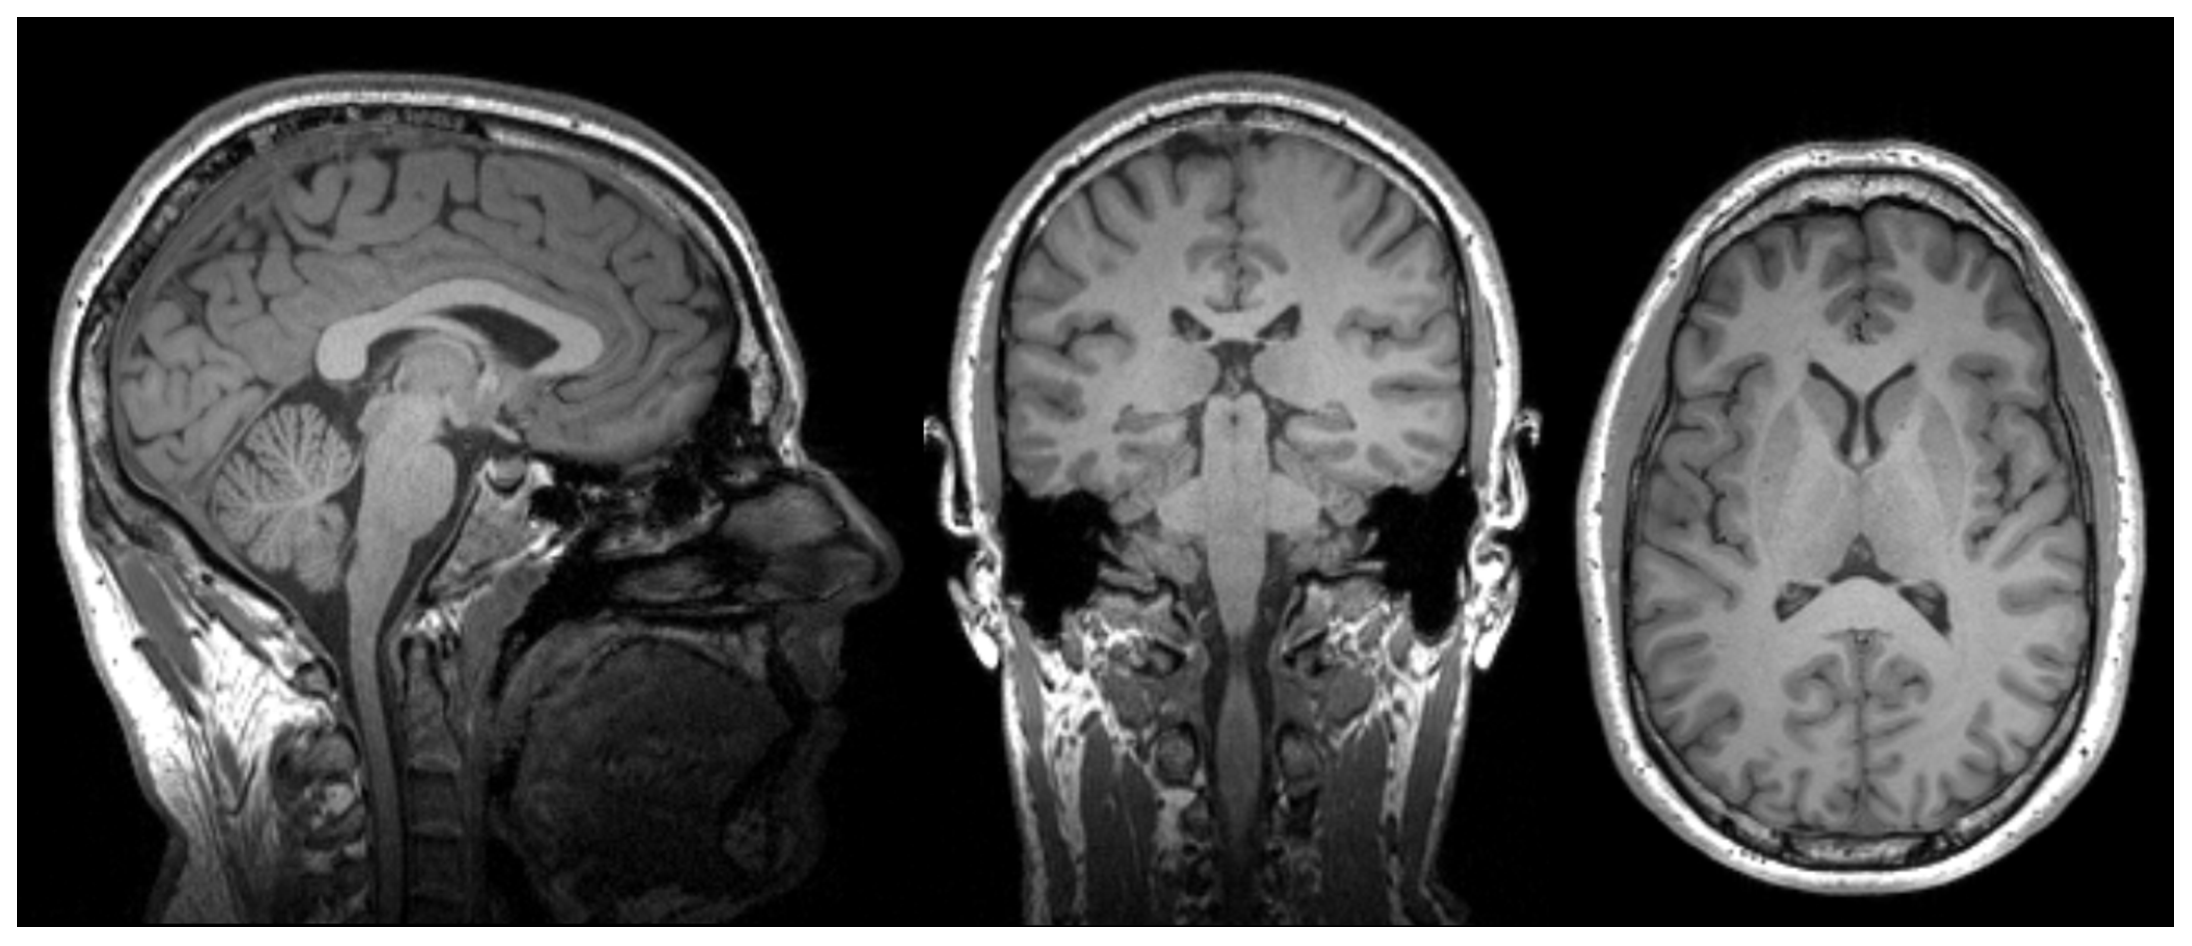
\includegraphics[width=0.7\linewidth]{Graphics/ch1/example_MRIT1}\\
	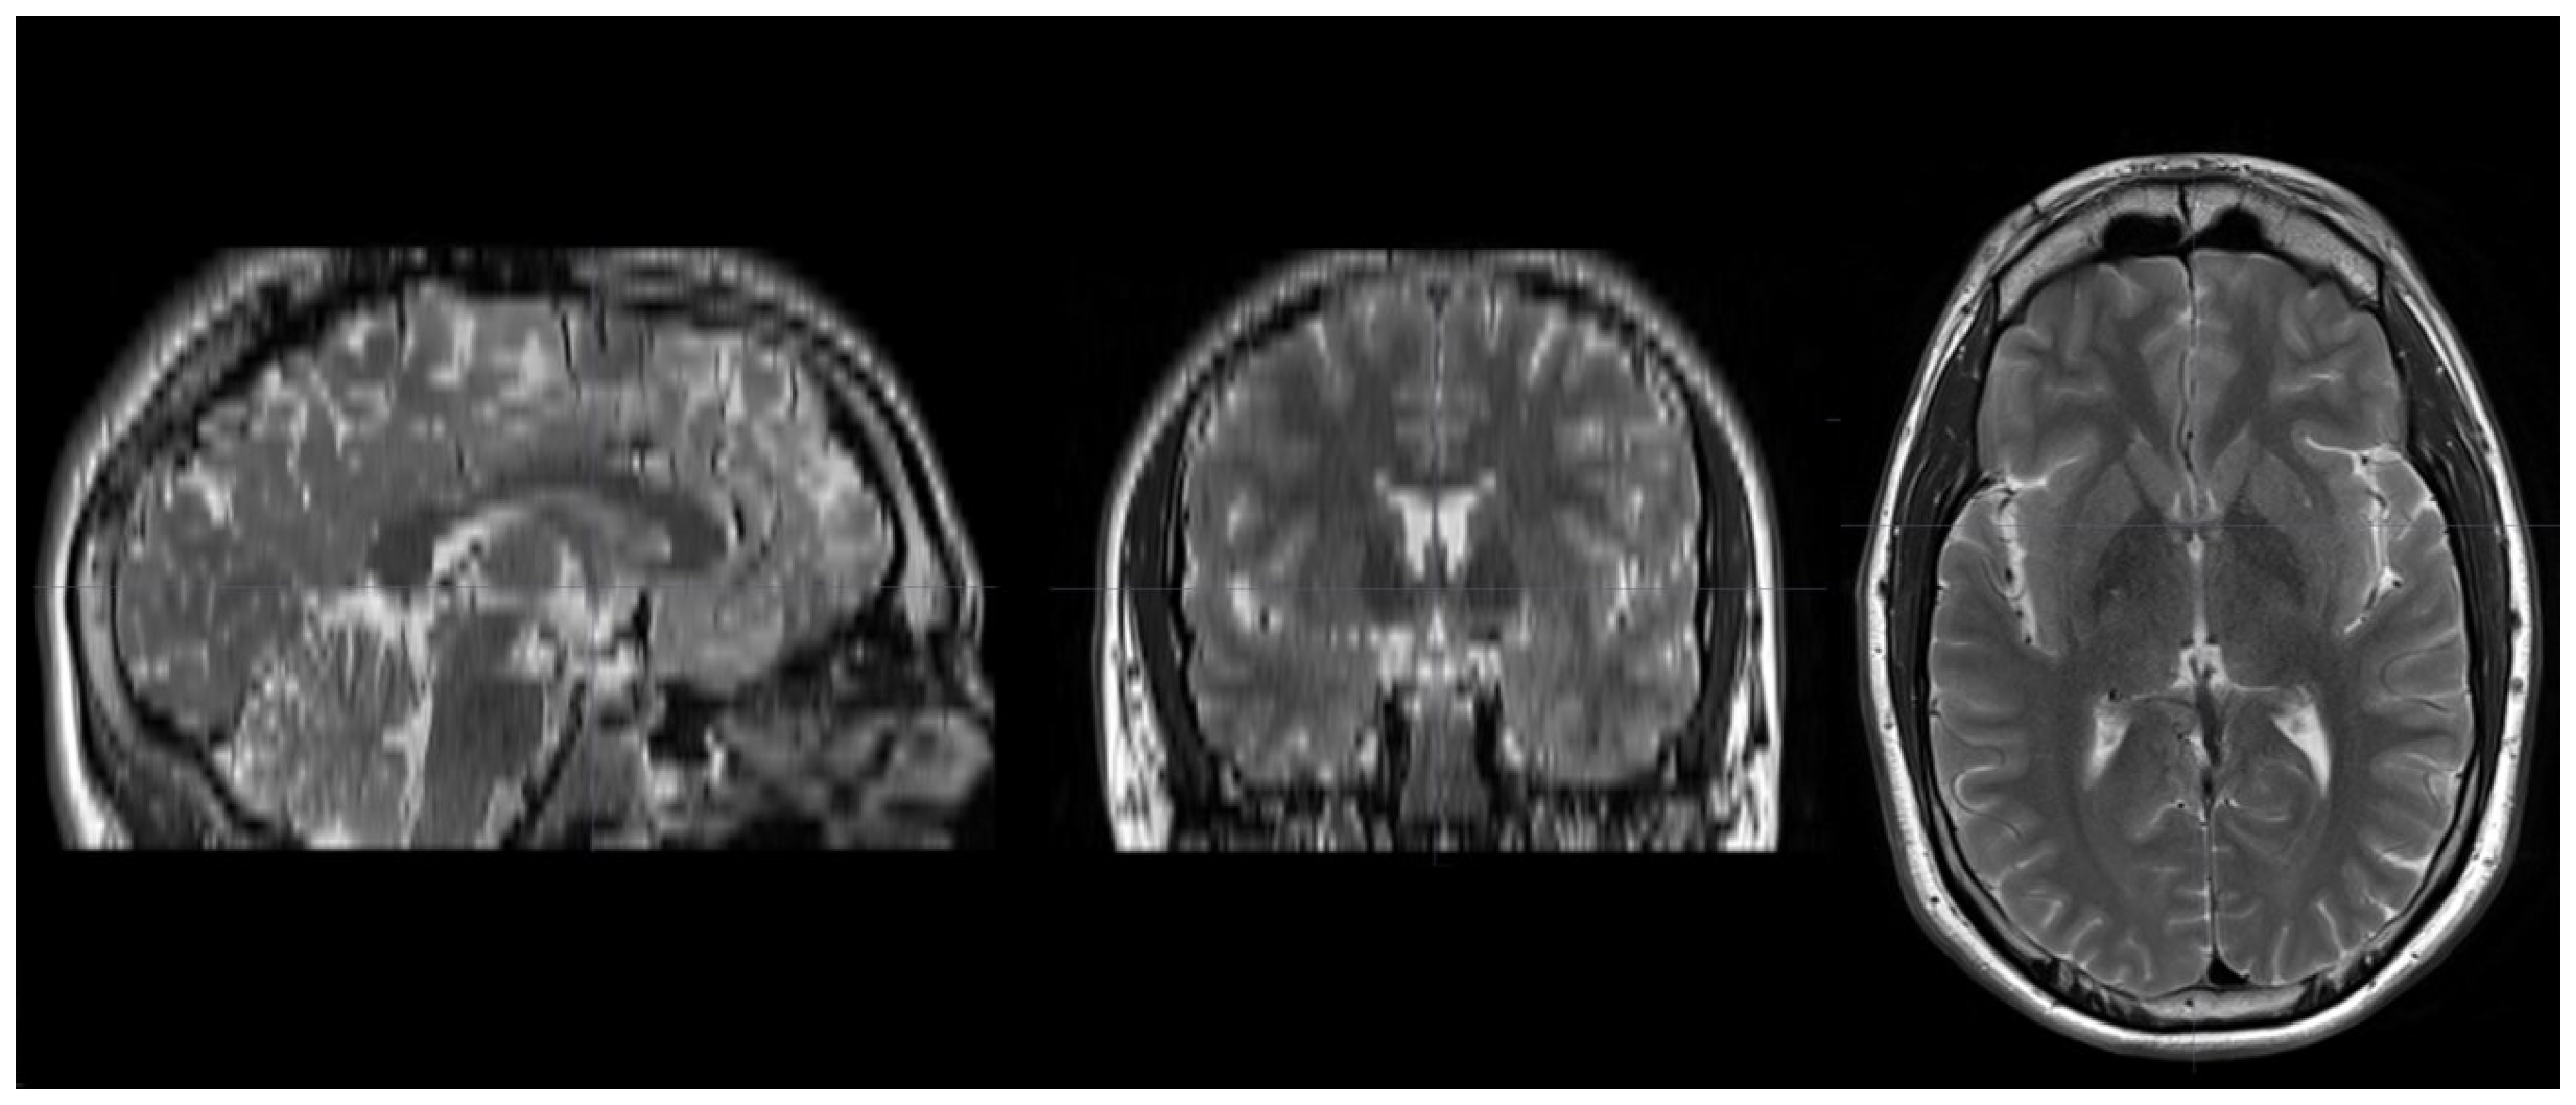
\includegraphics[width=0.7\linewidth]{Graphics/ch1/example_MRIT2}
	\caption[Example of T1 and T2-weighted MRI images.]{Example of T1 and T2-weighted MRI images of the same subject.}
	\label{fig:example_MRI}
\end{figure}

\ac{MRI} combines the magnetic field with a \ac{RF} emission to excite the atomic nuclei present in corporal structure, resulting in a image of the distribution of certain atoms in the body. Most \ac{MRI} use hydrogen atoms, since they are present in water (which adds up to around 70\% of body mass) and the signal derived is stronger than other atoms, increasing the \ac{SNR}, and therefore, the image quality. 

The procedure uses a strong magnetic field $B_0$ to align the magnetic moment of the hydrogen nuclei in parallel or anti-parallel (depending of their initial spin). This way, the magnetic moment of all nuclei will increase up to a stable state, in contrast to their null value in absence of $B_0$. Within this magnetic field, the hydrogen atoms precess around an axis along the direction of the field. 

A given nuclei has a resonance frequency which is proportional to the intensity of $B_0$, which, by using strong fields, allow us to resonate hydrogen far below potentially damaging frequencies. The precession frequency is determined by the Larmor equation (\ref{eq:lamor}):

\begin{equation}\label{eq:lamor}
f_0 = \frac{\gamma}{2\pi } B_0 
\end{equation}
where $\gamma$ depends on the nuclei, which in the case of hydrogen, $\gamma = 42.6$ MHz/T. When a subject is introduced in the \ac{MRI} scanner, it is submitted to the magnetic field $B_0$, so that the hydrogen nuclei are aligned to the field, with a precession frequency $f_0$. Then, a \ac{RF} pulse of the same frequency is generated, which is then absorbed by the nuclei, forcing them to place perpendicular to the field. Once the \ac{RF} emission is interrupted, the nuclei return to its equilibrium state by means of a procedure called relaxation. In this procedure, they emit part of the absorbed energy, which is then captured by a \ac{RF} receptor. Usually, position information is encoded in the \ac{RF} signal by varying $B_0$ using gradient coils. 

The \ac{RF} signal is measured during the relaxation time, and two different relaxation times are set: the T1 (spin-lattice) relaxation time and the T2 (spin-spin) relaxation time. The T1 time is the time during which nuclei emit energy to the adjacent tissue and realign to the longitudinal plane (z axis), whereas the T2 time refers to the time when nuclei realign to the transversal plane (y axis). These times are used to create T1-weighted and T2-weighted images (see Figure~\ref{fig:example_MRI}). T1-weighted images allow to distinguish between \ac{GM} and \ac{WM} in the cerebral cortex, to identify fatty tissue, and generally, obtain structural information. Conversely, T2-weighed images are used to assess \ac{CSF} or to visualize and identify \ac{WM} lessions. 

\subsection{Single Photon Emission Computed Tomography}
The \acf{SPECT} is based on the principles of \ac{CT}, by which a series of signal acquisition at different angles can be reconstructed back into a bidimensional distribution of the signal. In \ac{SPECT}, a gamma photon emitting radioisotope is linked to a pharmaceutical that binds to a given biomarker, generating a radiopharmaecutical or agent. This agent is injected into the patient, and after a certain time in which the radiopharmaceutical is distributed, the patient is introduced into the \ac{SPECT}-\ac{CT} scan. 

Afterwards, the scanner performs a series of acquisitions at different planes and angles from the body, from which the gamma signal is measured. For each plane, all acquisitions at each angle are pooled and a single two-dimensional image is reconstructed using a \ac{FBP} algorithm, or Radon inversion formula \cite{Herman2009l}, which derives from the Fourier's Theorem. A total of 180 projections per plane, using an angular resolution of 2 degrees, are usually taken. 

There exist a number of radiopharmaceutical used in clinical practice, and therefore, we will focus on the two varieties used in this thesis. First, we use an agent called $^{99m}$Tc-HMPAO, which consists of two stereoisomers of hexametazime (HMPAO) linked to the radioisotope technetium 99-metastable. This agent is usually used to assess \ac{rCBF}, which can be used to diagnose neurological diseases or cancer. 

\begin{figure}[htp]
	\centering
	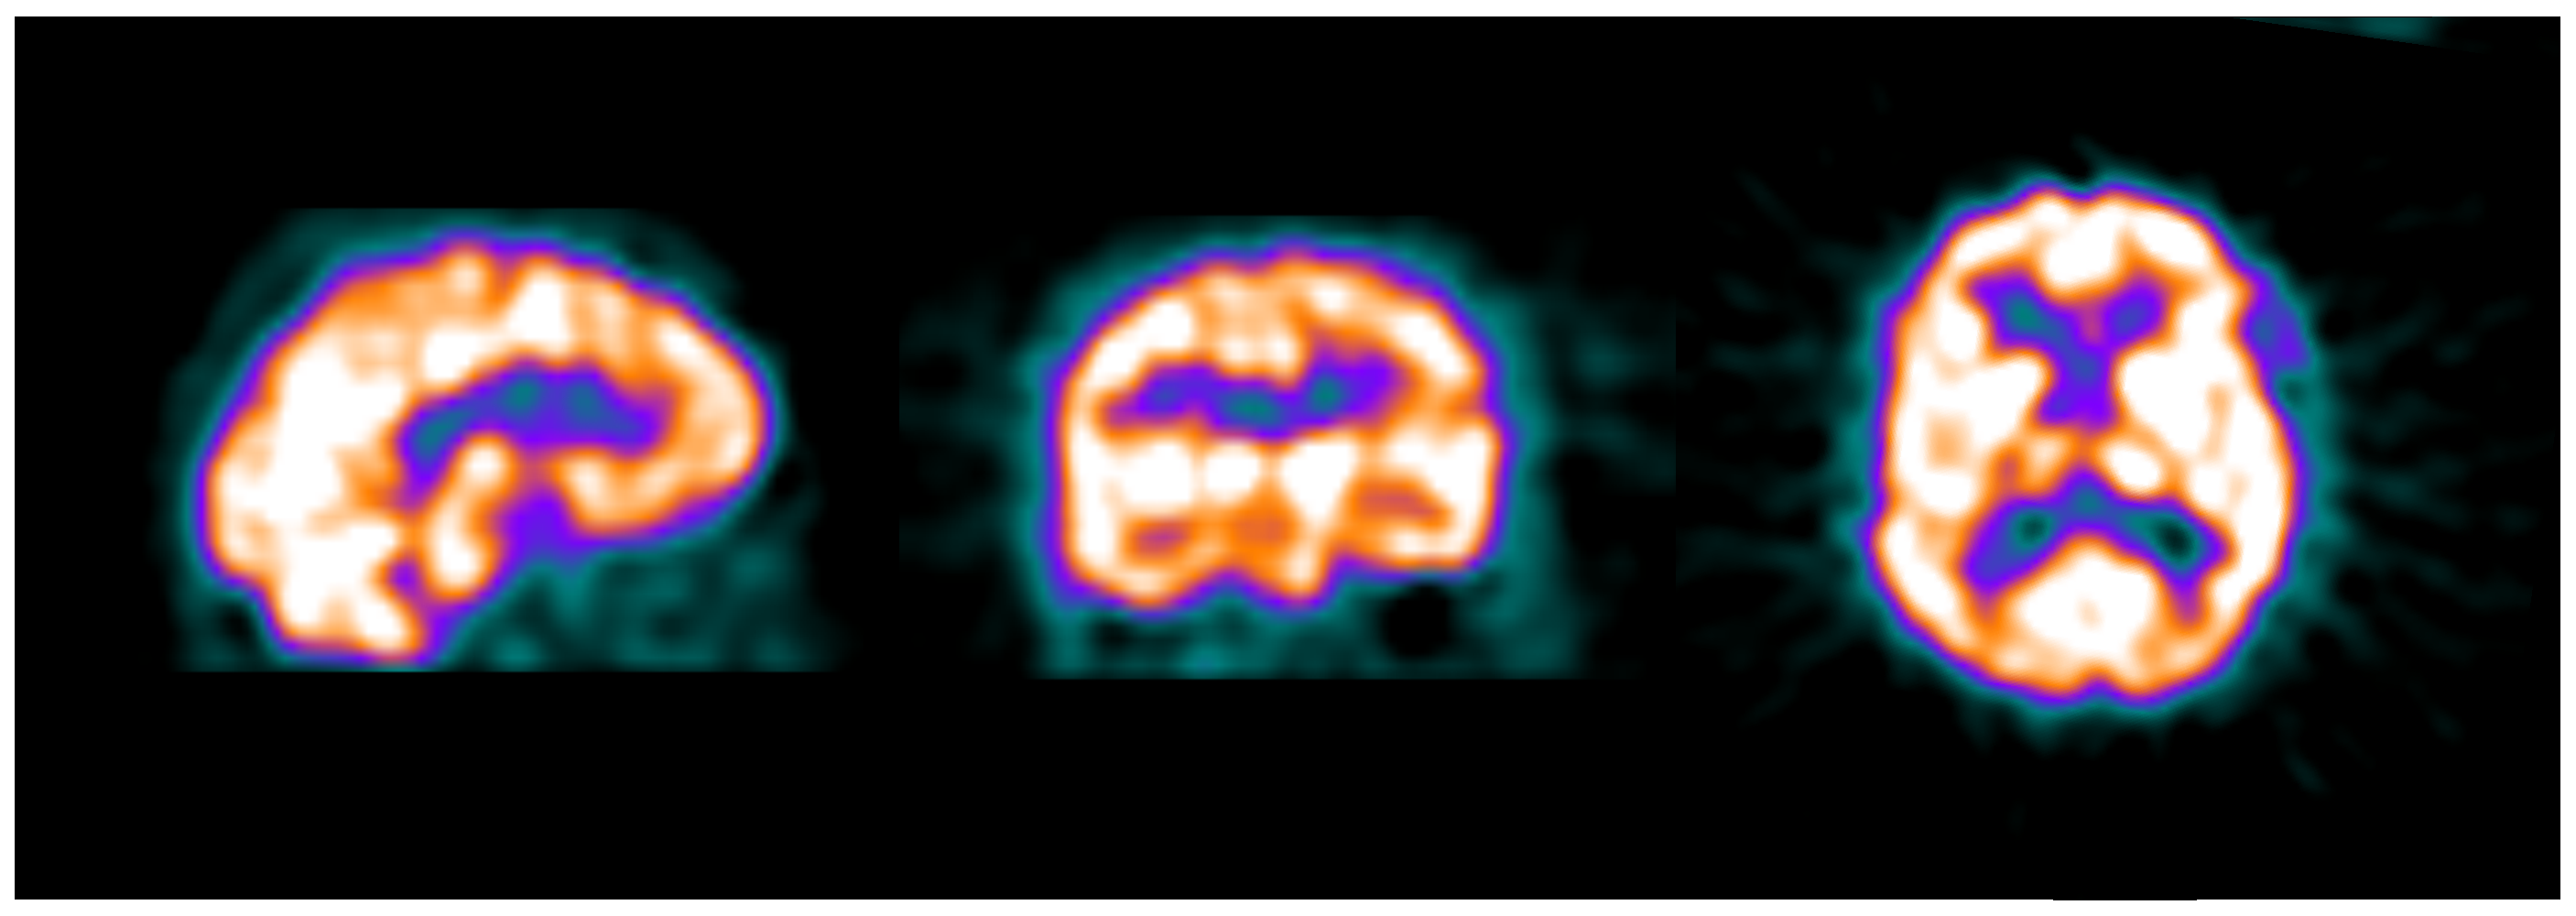
\includegraphics[width=0.7\linewidth]{Graphics/ch1/example_SPECT}\\
	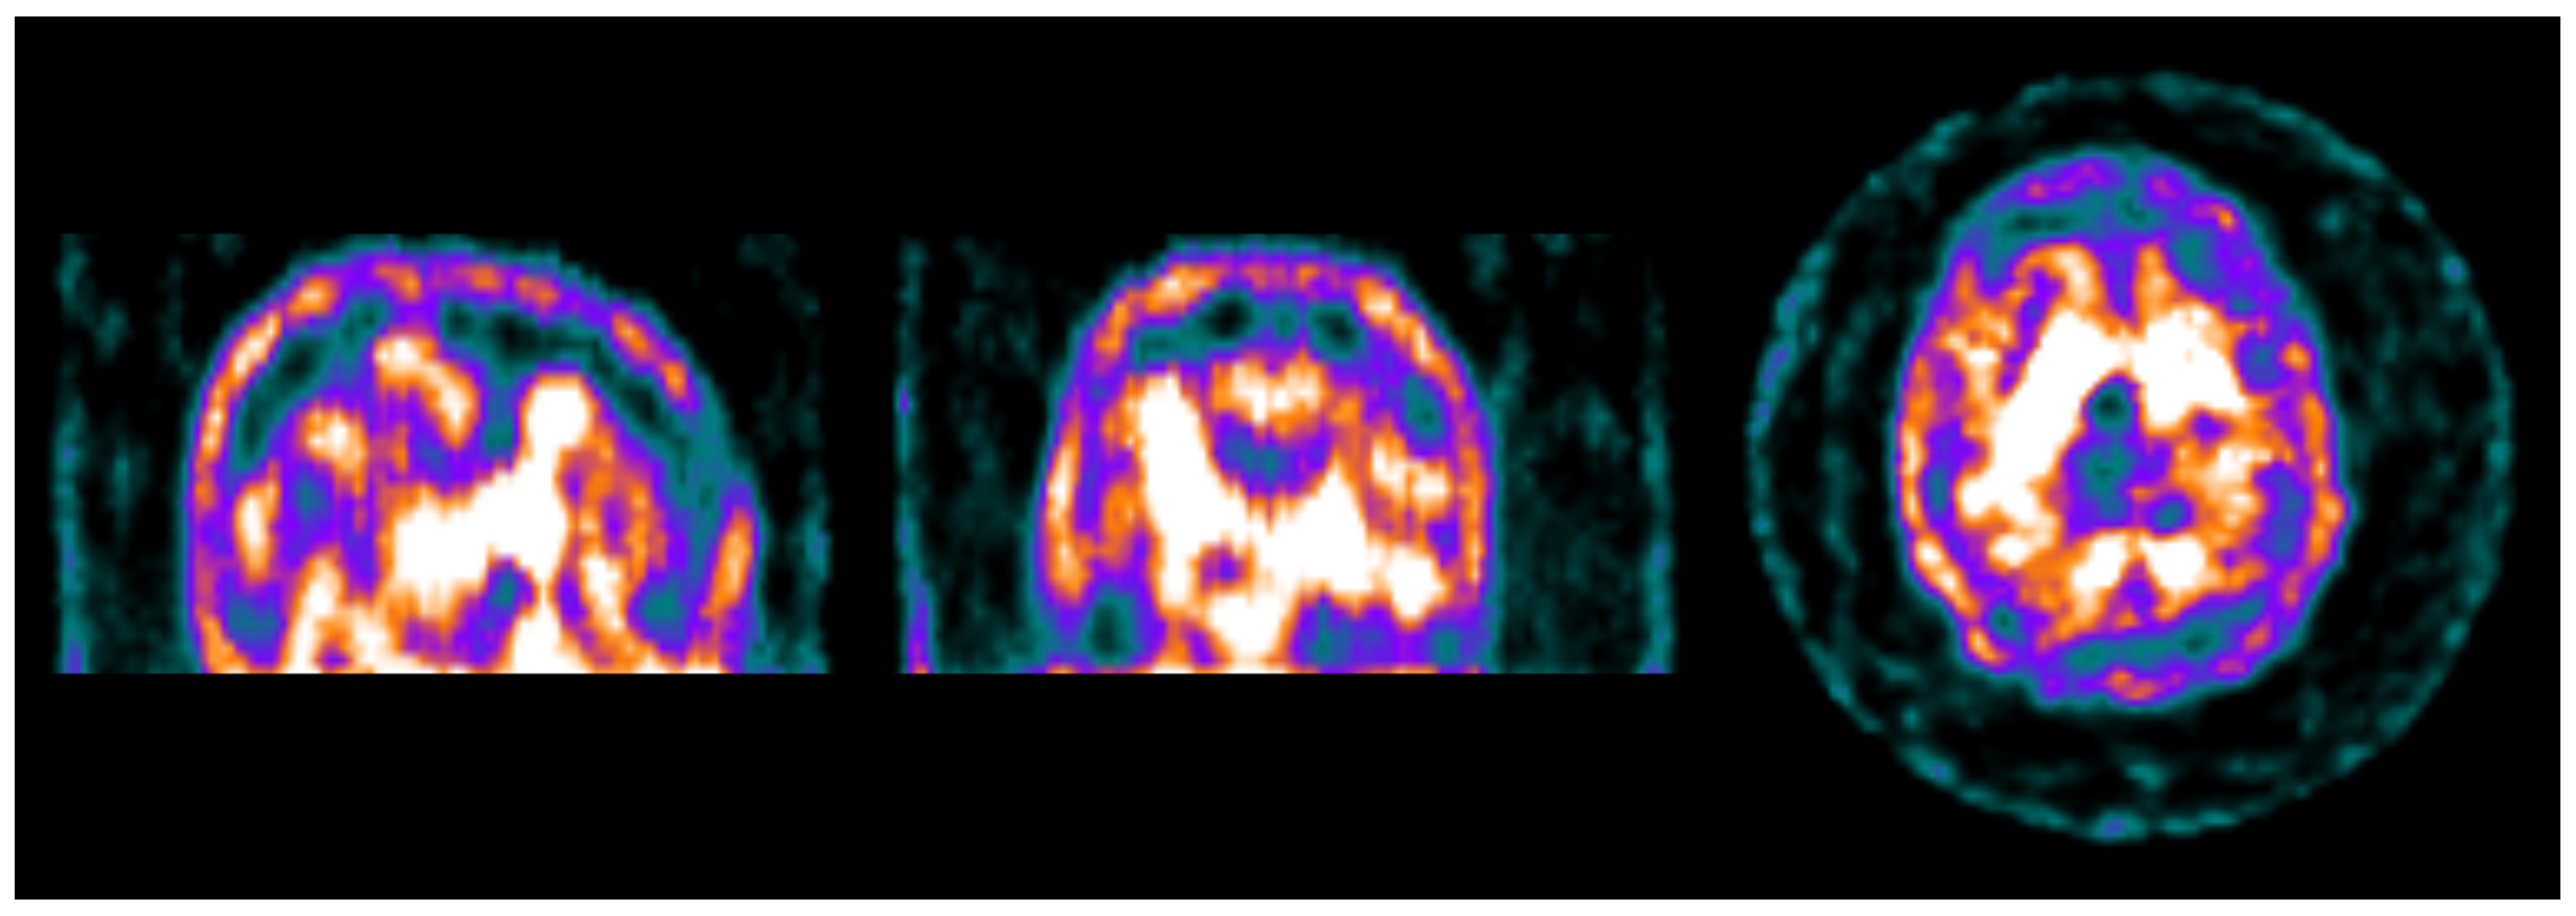
\includegraphics[width=0.7\linewidth]{Graphics/ch1/example_DaTSCAN}
	\caption[Example of SPECT images.]{Example of SPECT images, a SPECT-HMPAO and a SPECT-DaTSCAN.}
	\label{fig:example_SPECT}
\end{figure}

Additionally, we use images generated using the agent Ioflupane ($^{123}$I), a cocaine analog with high binding affinity for \ac{DAT}. It is used fundamentally in the assessment of \ac{PD}, given that the disease is associated with a loss of dopaminergic neurons in the striatal region. 

\subsection{Positron Emission Tomography}
The \acf{PET} is a technique similar to \ac{SPECT}, but in this case, the agent used and the equipment is designed to deal with a pair of gamma photons resulting of the annihilation of a positron with its corresponding antiparticle, the electron. The pair of photons are generated in opposite directions, and the detection depends on them being simultaneously or coincidently detected at the receptor. The receptor comprises a scintillator which emits light when the gamma photon incides, and a detector, usually a photomultiplier tube or silicon avalanche photodiodes.

It uses the same \ac{FBP} algorithm as \ac{SPECT} in the reconstruction of the images, and a similar strategy for acquiring the signal at different angles. However, the amount of data is smaller than in \ac{SPECT}, and therefore, the reconstruction procedure is harder. As a result, \ac{PET} scanner operation is considered more costly than \ac{SPECT} \cite{Carlson2016}.  

\begin{figure}[htp]
	\centering
	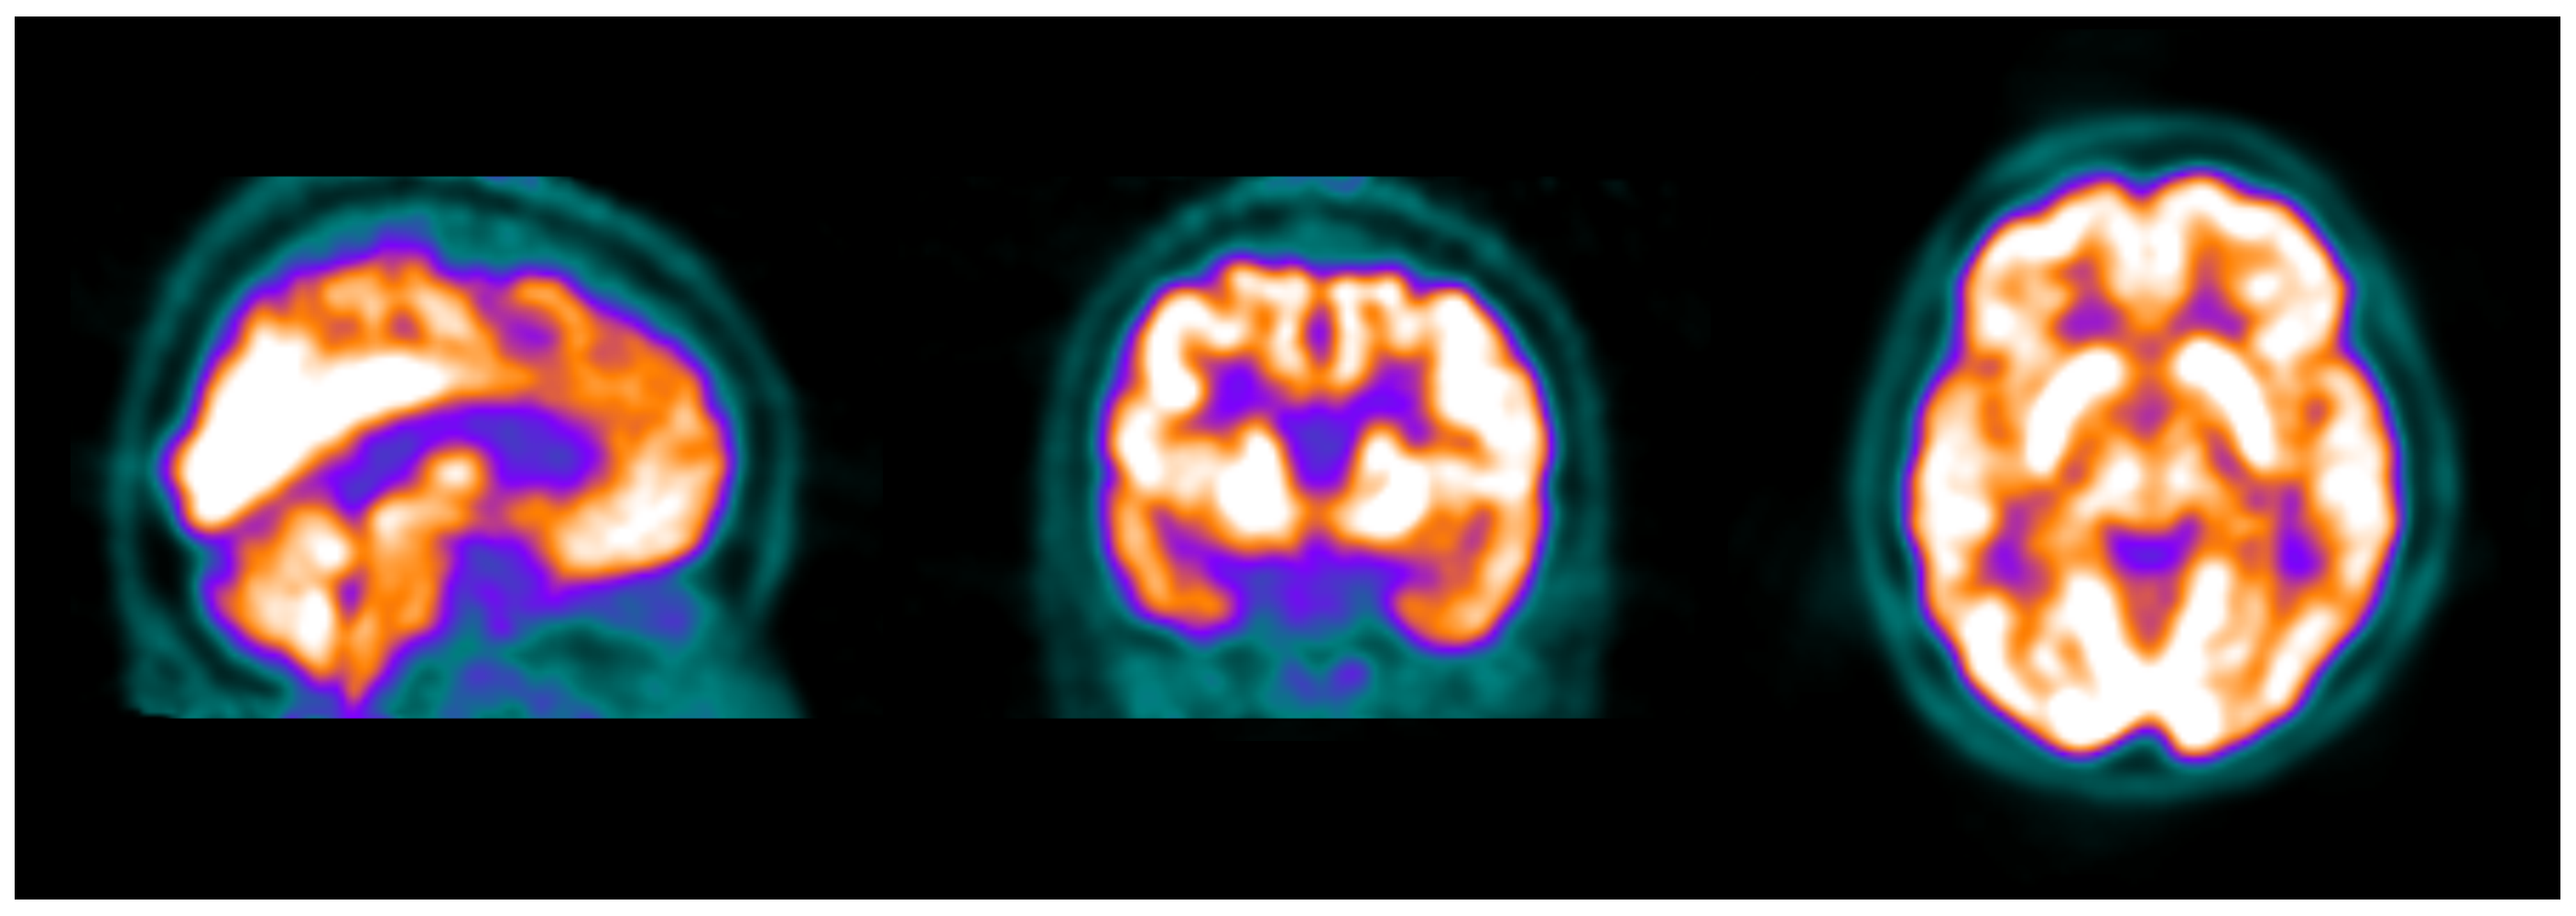
\includegraphics[width=0.7\linewidth]{Graphics/ch1/example_PET}
	\caption[Example of a PET-FDG image.]{Example of a PET-FDG image.}
	\label{fig:example_PET}
\end{figure}

The agent used in the images that we have processed is PET-FDG, also known as Fludeoxyglucose ($^{18}$F). It is a glucose analogue that allows us to measure the glucose metabolism in the brain. It is widely used in neurology \cite{Newberg2002} and cancer detection \cite{Kelloff2005}, since it can be correlated with cellular activity. 


\section{Voxelwise Analyses}
Traditional analysis of neuroimaging involves visual analysis by experts clinicians, or semi-quantitative analysis of \acp{ROI}. With the rise of neuroimaging in the mid-nineties, some computer-aided solutions appeared, starting with the widely known \acf{SPM} \cite{Friston1994}, its extension to structural imaging \acf{VBM} \cite{Ashburner2000} and later, the first application of classifiers to medical imaging, called \acf{VAF} \cite{Stoeckel04}.

\subsection{Statistical Parametric Mapping}
\acf{SPM} is a new methodology to automatically examine differences in brain activity in functional imaging studies involving \ac{fMRI} or \ac{PET}, firstly proposed by Friston in \cite{Friston1994}. The technique can be applied either to static images (e.g., \ac{PET}) or timeseries (\ac{fMRI}), using inference techniques based on hypothesis testing, in order to construct the \ac{GLM} that better describes the variability in the data. 

Statistical hypothesis testing involves constructing a pair of hypotheses: $H_0$, or the null hypothesis, that states no relationship between variables; and $H_1$, the alternative hypothesis. In neuroimaging, $H_0$ usually means that there are no relevant differences between classes (for example, between patients affected by \acf{AD} and \ac{CTL}), and $H_1$ implies that there is a significant difference. Many different tests such as massive univariate $t$-Test or \ac{ANOVA} (see Chapter~\ref{ch:decomposition} for more information on these techniques) can be used in the \ac{SPM} software \cite{spm_book}, by using a design matrix that describes a $t$ or $F$ based contrast (for $t$-Test and \ac{ANOVA} respectively). These terms are generally referred to as $Z$-values, namely the signed number of standard deviations an observation is above the mean. 

The test are computed voxel-wise, from which a $p$-value can be obtained, nominally the probability of obtaining equally or more extreme $Z$ values that the one actually found.
$p$-values are very extended in neuroimaging, representing the probability of a $Z$ value being equal or more extreme than the reference value given. In many studies $p < 0.05$ is used for measuring statistical significance, which means that only a 5\% of the times a experiment is repeated we would obtain that result or a more extreme one. The use of the significance threshold $\alpha=0.05$ implies that any voxel with a $p$-value smaller than 0.05 is considered sufficient to reject the null hypothesis. 

\begin{figure}[htp]
	\centering
	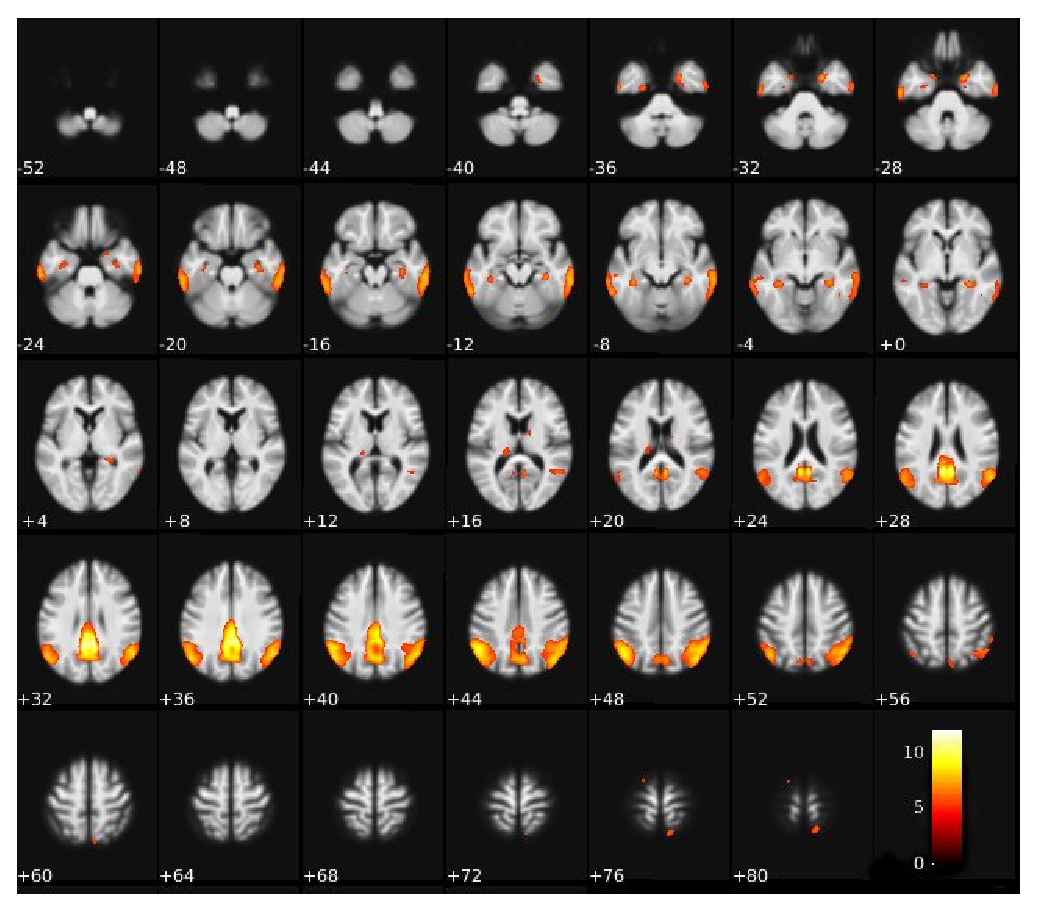
\includegraphics[width=\linewidth]{Graphics/ch1/example_SPM}
	\caption[Example of a \acs{SPM} analysis on a \acs{PET} dataset.]{Example of a \ac{SPM} analysis on a \ac{PET} dataset displaying the differences between \ac{AD} and \ac{CTL}, using $p<0.05$ and \ac{FWE} correction.}
	\label{fig:example_SPM}
\end{figure}

\ac{SPM} outputs maps like the one shown in Figure~\ref{fig:example_SPM}. There, significant $Z$-values according to a given threshold (\ac{FWE} uncorrected or corrected, see Section~\ref{sec:multiplecomparisons}) are displayed over an anatomical reference.  The resulting maps allow a visual inspection of the active brain areas, which can later be related to a certain disease or task. 

Although \ac{SPM}'s main feature is the estimation of differences, the term has been extended to cover the whole process performed by the \ac{SPM} software. That is, it generally involves registration to a template, intensity normalization, smoothing, the proper \ac{SPM} difference estimation and the display of the results. An overview of these procedures is provided at Chapter~\ref{ch:preprocessing}. 

\subsection{Voxel Based Morphometry}
\acf{VBM} can be considered an extention of \ac{SPM} applied to structural \ac{MRI} images \cite{Ashburner2000}. The procedure involves preprocessing (see Chapter~\ref{ch:preprocessing}), where smoothing is applied to reduce smaller anatomical differences. Afterwards, a \ac{GLM} is applied to each voxel in the images, and a $Z$-score map similar to Figure~\ref{fig:example_SPM} is produced. 

Smoothing is more important in \ac{VBM} than in regular \ac{SPM}, since \ac{MRI} images have higher resolution and are less noisy than functional images. Larger smoothing kernels will miss out smaller regions, while smaller kernel can lead to artifacts in the generated $Z$-maps, including misalignment of brain structures, differences in folding patterns or misclassification of tissue types \cite{Martinez-Murcia2016book}. Therefore, the kernel size must be carefully chosen, usually using a-priori knowledge about the regions affected, and always double checking for artifacts and reproducibility. 

The idea behind \ac{VBM} has been extended in a number of papers, using multivariate approaches that takes into account all voxels at once, and not their individual differences. Some of them include \ac{ICA} decomposition of the dataset and a posterior conversion to $Z$-scores in what was called Source Based Morphometry \cite{xu2009source}, or multidimensional Tensor Based Morphometry \cite{bossa2010tensor}. 
\subsection{The Multiple Comparisons Problem}\label{sec:multiplecomparisons}
The Multiple Comparisons problem arises when using hypothesis testing to assess statistical significance. This is widely used in neuroimaging, where statistical tests such as the $t$-Test or \ac{ANOVA} are used to quantify voxel-wise differences, and state their statistical significance, or $p$-value. The $p$-value, as described above, is the probability of any value being more extreme than a certain threshold under a given hypothesis. In our problem, given the $t$-value $T_i$ for the $i^{th}$ voxel ($i=1,\dots N$) of the images, and a threshold $T_{th}$ under the hypothesis $H$, the significance can be assessed by checking:
\begin{equation}\label{eq:pvalue}
P \left(T_i > T_{th}| H_0\right)<\alpha
\end{equation}
where $\alpha$ is the significance level. 

Choosing $\alpha$ is not trivial in neuroimaging. The use of the significance level $\alpha=0.05$ implies that any voxel with a $p$-value smaller than 0.05 is considered sufficient to reject the null hypothesis. This does not directly imply the necessity of accepting the alternative hypothesis $H_1$, although it is often thought so. Neither it yields the probability of the null hypothesis \cite{Dixon2003}. 

If we apply $p<0.05$ directly to a medical image of, for example, 300,000 voxels, that could mean the possibility of almost 15,000 voxels being false positives. Controlling the apparition of false positives when applying a massive univariate test is not trivial. It implies a balance between the true positive rate (sensitivity) or true negative rate (specificity), given that, for example, controlling the amount of false negatives will result in many false positives and vice-versa. 

Usually, two options for controlling the amount of false positives are given: the \acf{FWE} and the \acf{FDR}. The \ac{FWE} is the probability of obtaining at least one type I error. Mathematically, the null hypothesis for the $i^{th}$ voxel $H_{0i}$ states that there is no activation in that voxel. Therefore, the family-wise null hypothesis for our problem is:
\begin{equation}
H_0 = \bigcap_i H_{0i}
\end{equation}

If we reject a single null hypothesis ($T_i > T_{th}$), we reject $H_0$. Therefore, we want to control the probability of a single voxel being significant if the family-wise null hypothesis is valid:
\begin{equation}
P \left(\bigcup_i\{T_i > T_{th}\} | H_0\right)< \alpha
\end{equation}

In this case, we must obtain the critical value $T_{th}$, which is the higher $t$ value that matches that expression. Many options have been proposed to this problem, among them the conservative Bonferroni correction, methods that use random field theory or permutation tests. 

\subsubsection{The Bonferroni Correction}
The Bonferroni correction \cite{Shaffer1995} rewrites eq.~\ref{eq:pvalue} setting $\alpha=\frac{\alpha}{N}$ so that: 

\begin{equation}
P \left(T_i > T_{th}| H_0\right)< \frac{\alpha}{N}
\end{equation}

That way, using the Boole's inequality:
\begin{equation}
FWE \leq \sum_{i}^{N} \frac{\alpha}{N} = \alpha
\end{equation}

Therefore, we can comply with the imposed restriction for a maximum \ac{FWE}, or in our case, a maximum rate $\alpha$ of false positives. This is considered a rather conservative approach. In the example cited above, if we want to keep the \ac{FWE} below $0.05$, we should divide it by $N$, therefore obtaining a $T_{th}$ that makes $\alpha = 0.05/N = 1.67\times10^{-7}$. 

Other less conservative options try to compute a critical value $T_{th}$ that minimizes the \ac{FWE} using spatial information. This is the case of using an approximation of the distribution of the maximum statistic over the image, or the spatial correlation, including elements from random field theory (the approach used in \ac{SPM} \cite{spm_book}). 

\subsubsection{Random Field Theory}
In the random field approach, the maps of the statistic are treated, under the null hypothesis, as a lattice representation of smooth isotropic three dimensional random fields of test statistics. This approximation to the problem allow us to approximate the upper tail of the maximum distribution, the part needed for defining an event that occurs when the map exceeds the critical value $T_{th}$. Further information about random field theory and how it is applied to neuroimaging can be found at \cite{spm_book}. 

The other approach, based on the \ac{FDR}, aims at controlling the proportion of false positives in the total number of voxels declared significant. The most extended procedure for controlling the \ac{FDR} is that proposed by Benjamini and Hochberg \cite{Benjamini1995}. The Benjamini and Hochberg method start with calculating the $p$-values of all voxels and ranking them so that:
\begin{equation}
p_1 \leq p_2 \leq \dots \leq p_i \leq \dots \leq p_N \quad \forall i=1\dots N
\end{equation}

\subsubsection{FDR Controlling Procedures}
Let $q$ be the a maximum \ac{FDR} value that we can afford, for example $0.05$. For each $i$, we compute:
\begin{equation}\label{eq:bhFDRineq}
p_i \leq \frac{i}{N}q
\end{equation}

The maximum $i$ value that holds Eq.~\ref{eq:bhFDRineq} is used as $\alpha$, the significance level, and its corresponding statistical value ($T_i$ in the case of a $t$-test) is used as the critical value. This test, under the family-wise null hypothesis $H_0$, is equivalent to controlling the \ac{FWE}. However, \ac{FDR} methods are less conservative than other approaches such as the Bonferroni or other \ac{FWE}-based corrections, leading to a gain in statistical power. 


\subsubsection{Permutation Tests}
An empirical way to obtain $p$-values without relying on any parametric assumption is permutation testing \cite{Anderson2001,Winkler2014}. Permutation tests evaluate a statistic such as the F-statistic or the $t$-test using randomly target variables, in our case, the classes. The procedure is applied many times (up to 10,000), and for each permutation, only the maximum value of the computed statistic is considered. These values are used to build the null distribution, from which the family-wise corrected $p$-values are computed. We assume t

Results obtained in permutation tests are comparable to those obtained using Random Field Theory \cite{Winkler2014}, and far less conservative than when applying the Bonferroni correction. Many permutation schemes can be applied. The one that we use here is based upon \cite{Anderson2001}, as it was demonstrated to achieve more sensitivity than other alternatives. 

\section{Machine Learning in Neuroimaging}\label{sec:machinelearning}
In recent years, many efforts have been put into discovering new automatic or semi-automatic algorithms for analyzing neurological images, in has been known as \acf{CAD}


\subsection{Voxels as Features}
Another voxel-wise approach, involving the use of classifiers, is \acf{VAF} \cite{Stoeckel04}. It was firstly proposed for evaluating and performing automatic diagnosis of \ac{AD} using functional \ac{SPECT} imaging. It is the simpler machine learning approach used in this thesis, using a standard preprocessing (registration, intensity normalization) and a \ac{SVC} (See Appendix~\ref{ch:svm}) to predict the class of an image using all its intensities as features. 

It has been used in many works as a baseline \cite{Salas-Gonzalez2009}, since it is comparable to the performance achieved by expert physicians using visual analysis \cite{Stoeckel04}. The weight vector of the \ac{SVC} can be inverse transformed to the dimension of the original images, and therefore provide a visual map that reflects the most influential voxels, in a similar way to the $Z$ maps of \ac{SPM} and \ac{VBM}. 

\subsection{Multivariate Analyses}
In contrast to traditional visual inspection a semiquantitative analysis of neuroimaging, machine learning is nowadays a trend in the field. Machine learning is the subfield of computer science that provides computers with the ability to learn from data instead of being programmed for an explicit task. Applications range from automatic processing of images to , 

Statistical techniques such as \ac{PCA}, are used for feature extraction and hypothesis testing for feature selection in systems intended to 

This thesis explores how to use signal processing and machine learning to overcome the small sample size problem in neuroimaging. 

\ac{CAD}

The application of new machine learning techniques in CAD systems is a current trend. Works on this topic have increased exponentially in the past ten years, and it is expected to grow even more. Machine learning explores the study and construction of algorithms that can learn from and make predictions on data, and therefore, it is very useful in neuroimaging. 

Two approaches exist in machine learning. Supervised learning explores the patterns that lead to a certain outcome, e.g. the brain activation patterns that are related to a certain disease. On the other hand, unsupervised learning explores the underlying structure of the data. Machine learning in CAD is mostly based on supervised learning, since it is focused on the prediction and analysis of patterns related to a certain disease. 

In its simplest form, a machine learning pipeline for neuroimaging consists of a single classifier, just as the VAF approach that we mentioned. However, classifiers can improve their detection power if higher level features are extracted from the data, e.g., features that represent the distribution of the voxel intensities, the texture of the images, or the sources of variance of the maps. This is known as feature extraction, and the most common technique is image decomposition. 


